\appendix 
\thispagestyle{empty}
\hypertarget{AppendixB}{}\section*{Appendix C: Simulation tools} 



Developing an MVS necessitates utilizing accurate simulation tools. These tools typically provide confident vehicle models and environments, which are well-suited for analyzing, validating, and optimizing autonomous systems. In \cite{tong2020overview}, the authors conducted a comprehensive review of the latest advancements and analyses concerning simulation tools.



The algorithms proposed in this PhD study underwent testing within a simulation environment. Specifically, the decision, planning, and control modules of the C-MCA framework were developed using Matlab (cf. Figure \ref{fig:simulation_tool1}), with the simulation executed through Simulink.

Initially, the Unreal Engine 3D was employed to recreate the on-ramp merging scenario. To bridge the gap between Simulink and the Unreal Engine, a connecting interface was established, facilitating the integration of the simulation and 3D components, such as vehicle motion. In the Unreal Engine tier (see Figure \ref{fig:simulation_tool1}), the 3D model and environment utilized for the simulation were constructed based on the Unreal Engine platform. The simulation environment represents a response to the on-ramp merging scenario within the module, with virtual vehicles comprising models of the vehicles and sensor modules. Lastly, the bridge module facilitates communication between Simulink and the Unreal Engine tier.




        \begin{figure}[!h]
        \centering 
        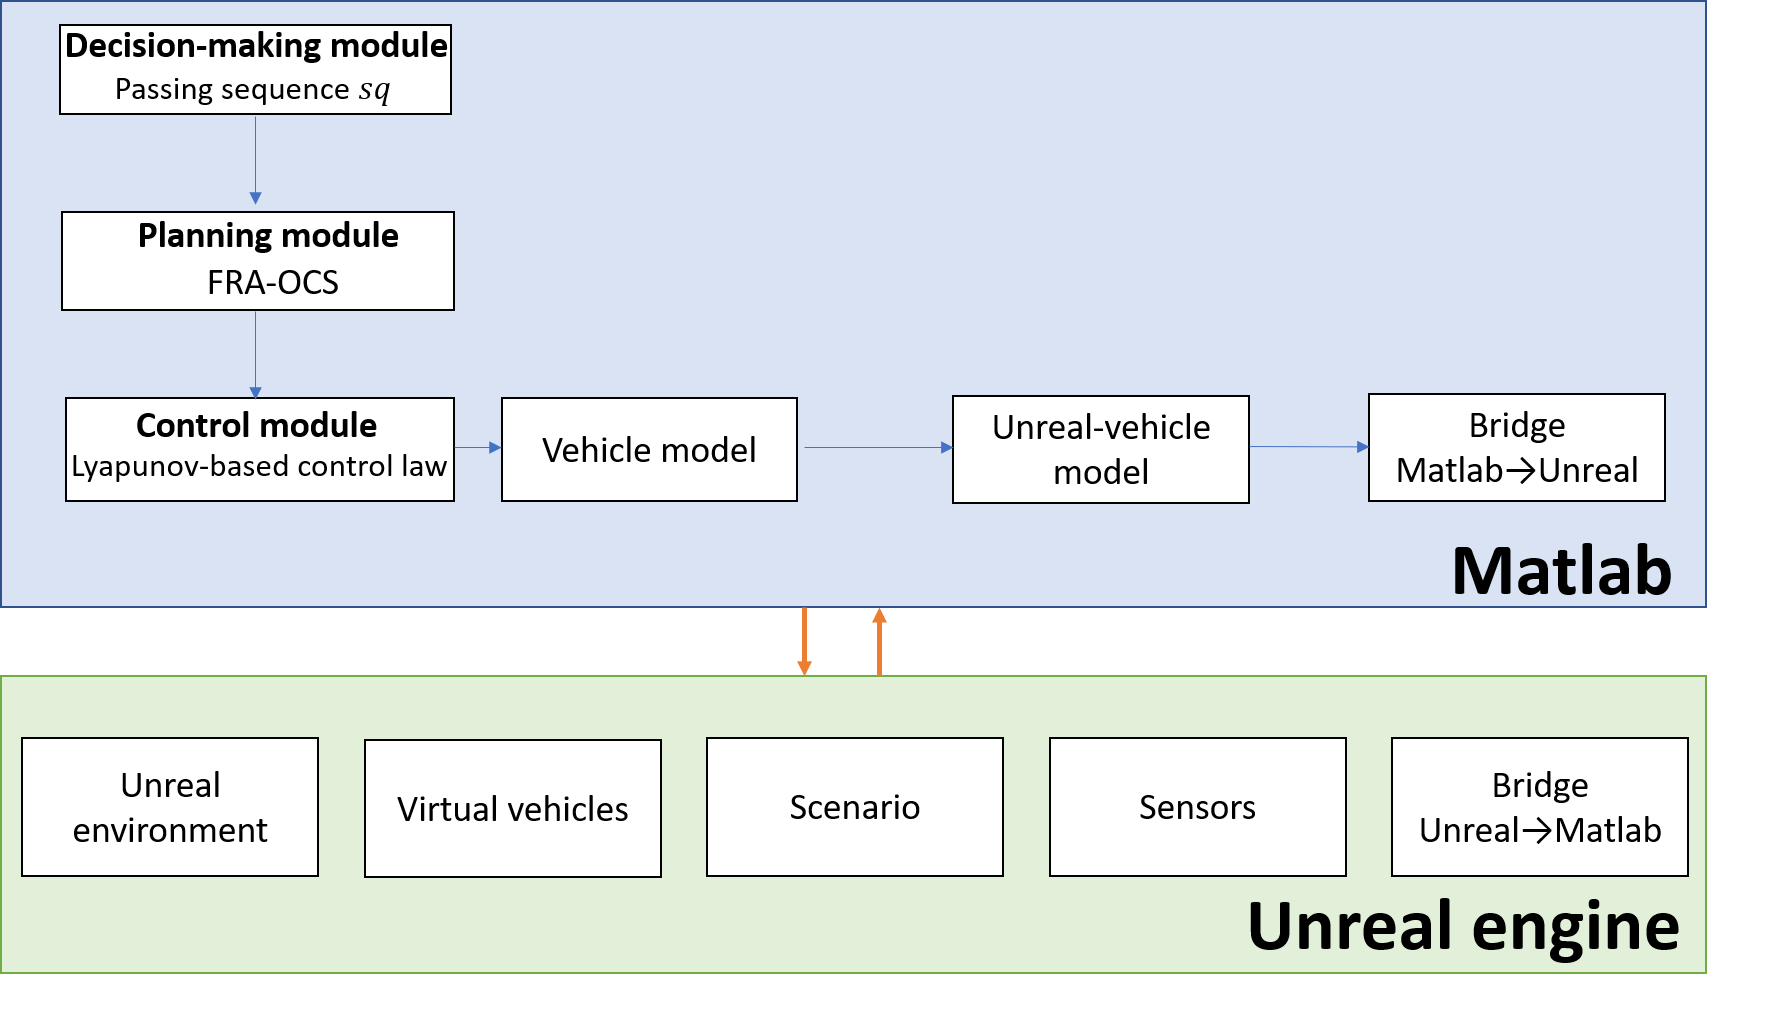
\includegraphics[width=11cm,height=18cm,keepaspectratio]{appendices/Slide_sup1.png}
       % \vspace{-2.3mm}
        \caption{The overall simulation architecture  }
        \label{fig:simulation_tool1}
       % \vspace{-5mm}
        \end{figure}

The virtual vehicle module within Unreal Engine employs a kinematic vehicle model, which represents a significant limitation. To address this drawback, SCANeR studio was utilized. Besides its integration of an advanced dynamic model of the vehicle. SCANeR stands out as one of the most comprehensive solutions for automotive simulation, enabling users to configure, prepare, execute simulations, and analyze outcomes effectively. Its versatility proved especially valuable for scenarios involving multiple vehicles, such as MVS. Integration of the SCANeR studio simulation solution followed the same architectural framework as previously depicted (refer to Figure \ref{fig:simulation_tool2}).

        \begin{figure}[!h]
        \centering 
        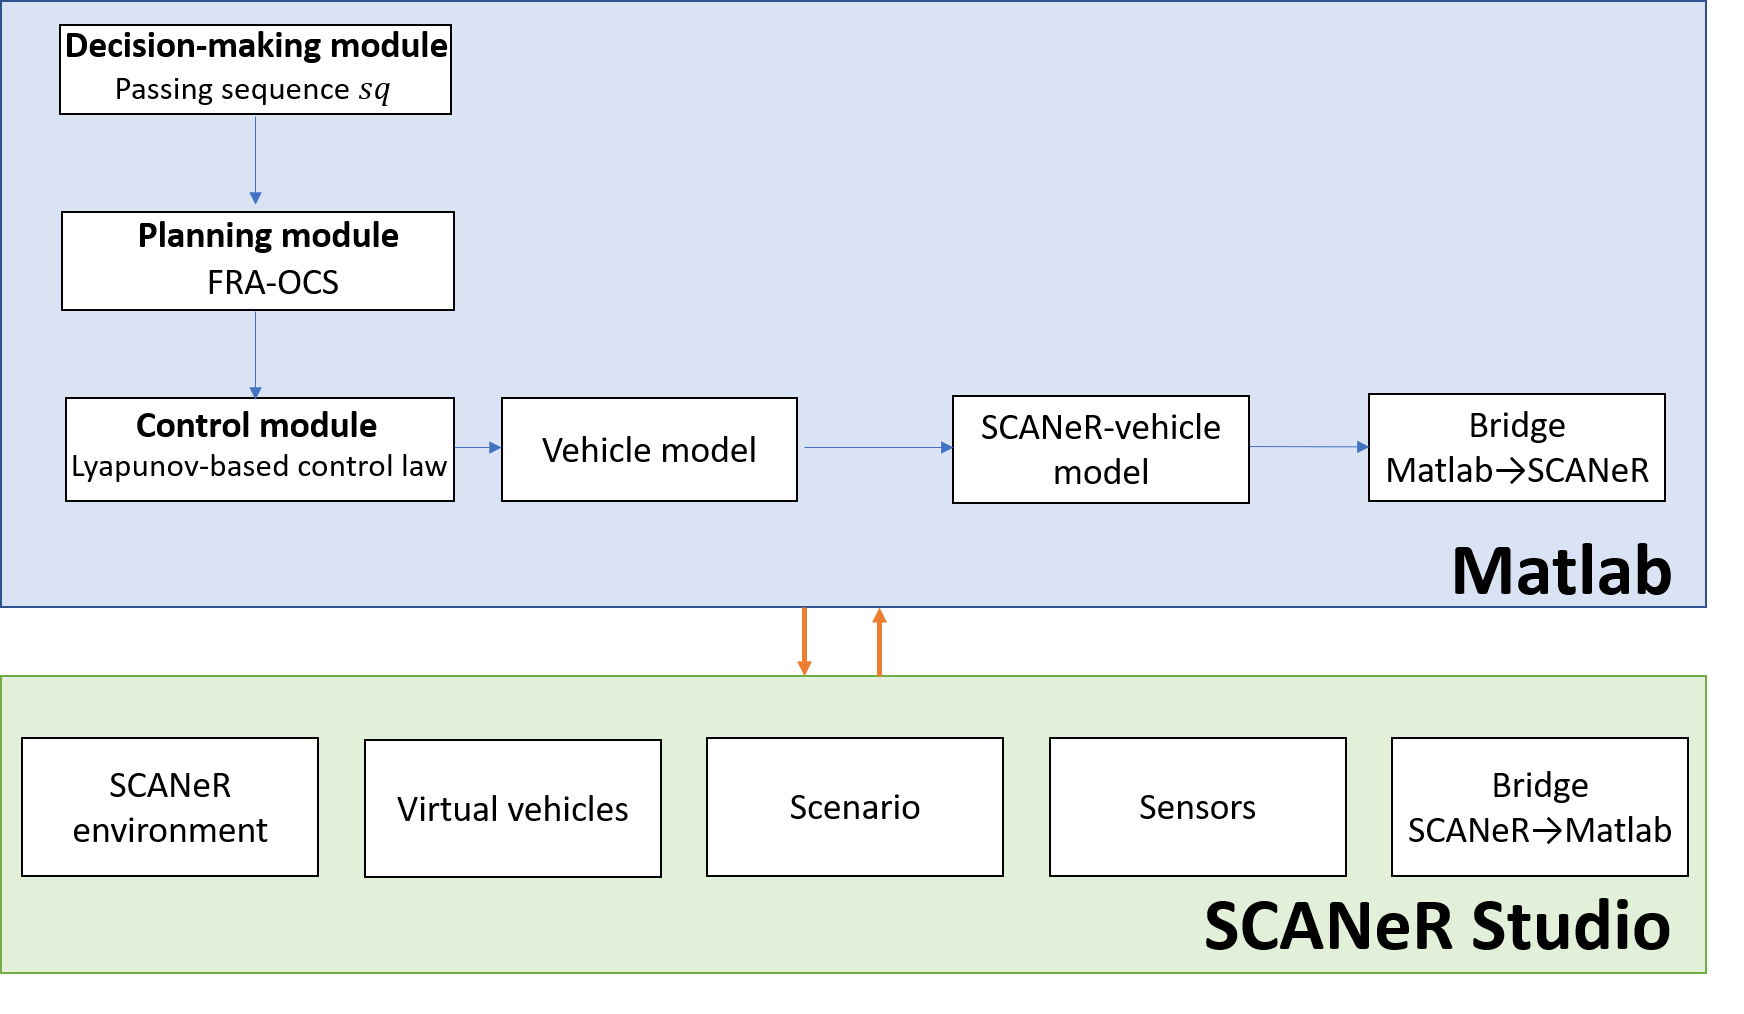
\includegraphics[width=11cm,height=18cm,keepaspectratio]{appendices/Slide_sup2.png}
       % \vspace{-2.3mm}
        \caption{The overall simulation architecture  }
        \label{fig:simulation_tool2}
       % \vspace{-5mm}
        \end{figure}